\documentclass{article}
\usepackage{url}
\usepackage[utf8]{inputenc}
\usepackage{graphicx}
\usepackage{collcell}
\usepackage{listings}
\usepackage{amsmath}
\usepackage[margin = 0.75in]{geometry}
\usepackage{xcolor}

% Defines the colors that are used
\definecolor{comment_color}{rgb}{0,0.6,0}
\definecolor{number_color}{rgb}{0.5,0.5,0.5}
\definecolor{string_color}{rgb}{0.58,0,0.82}
\definecolor{backcolour}{rgb}{0.95,0.95,0.95}
\definecolor{nvidia_green}{HTML}{76b900}

% This is here in case we want to include code in the future
\lstdefinestyle{mystyle}{
    backgroundcolor=\color{backcolour},   
    commentstyle=\color{comment_color},
    keywordstyle=\color{magenta},
    numberstyle=\tiny\color{number_color},
    stringstyle=\color{string_color},
    basicstyle=\ttfamily\footnotesize,
    breakatwhitespace=false,         
    breaklines=true,                 
    captionpos=b,                    
    keepspaces=true,                 
    numbers=left,                    
    numbersep=5pt,                  
    showspaces=false,                
    showstringspaces=false,
    showtabs=false,                  
    tabsize=2,
    frame=tb
}

\lstset{style=mystyle}
\graphicspath{./imgs}
\title{Musically Composed Visuals-Draft}
\author{Fourier2 Team}
\date{Spring 2023}

\begin{document}

\maketitle

\section{Team}
Justin Choi, Ryan Gaffney, Ian Lips, Matt Dim

\begin{enumerate}
\item Our project is going along very well. We have the basics of audio processing that takes a wav file and performs the fourier transform. We also have managed to create an output of a visual based on our transformed audio. While we still need to work on more utilization of parallelization and connecting our programs coherently, I would give us a score of \textbf{4} on our progress.
\item I would say we require \textbf{Normal} feedback, as we have our plans and steps set for our implementation, yet if there are any glaring issues with the setup of our project it would be nice to know before committing further.
\item Our group has no issues in finding times to work and have meetings for our project. \textbf{Great}
\item At the moment I don’t believe we have any questions
\end{enumerate}

\section{Overview}
\par Our starting point for this project had two main topics, audio processing with fourier transform, and displaying an image from a julia set given an input. For the audio, our start consisted of a lot of research on how people process audio into a format to where we can use it as an input for our image generation. While we already knew we would perform fourier transform we still needed to understand what our initial audio would start as, and how the processing would result in a data type that can be transformed with fourier. After looking through several different ways of audio processing, we decided to go with the format of using wav files with FFT (fast fourier transform) processing. We will be able to parallelize this using OpenMP to perform the transformation across many threads. In order to deliver the information to our image generator, we decided to use a CSV format in order to feed our processed audio into the visualizer.

\section{Fast Fourier Transform (FFT)}
\par A lot of our time was used for researching and discovering libraries that we could utilize for our project. We knew that we would use OpenGL for our visualization, but for audio processing there are several different ways we could have gone about it. Thus, most of our time was not spent on implementation, but was used to understand how libraries worked and which libraries would be good candidates for our needs. We found multiple libraries in c and c++ that we have decided to utilize in our file conversion, signal processing, and graphics which will be included in our references. 
\par The fourier transform output essentially keeps track of all the frequencies like a histogram of a song, and creates a magnitude to see how many times that frequency appears in a given song. We decided to use the wav file format for our implementation due to how they are easier to parse through for processing. MP3 files are compressed which results in smaller files as data is lost from compression. Going with this implementation was the most optimal way to create a format to easily input into our visualizer. The most difficult part of this initial draft was finding ways of integrating the two parts of our program. Building the visualizer, we had a difficult time understanding input, alongside a way of creating outputs of our audio processing. 
\par Looking back at our Draft Deliverable, we have met a lot of the requirements set for ourselves. We have successfully gotten a song in wav format to be broken down and fed to an audio visualizer. However, there have been significant issues with trying to parallelize our fast-fourier transform. We’ve been trying to use OpenMP to try and get a noticeable speedup in computation. For now we have only noticed the program actually slowing down in real practice, so that part of the deliverable I think was a little too optimistic to have done at this time in the project. The code we’ve ended up with does output an image from song data, but I believe we would like to make a modification in getting the parallelization done with OpenMP and Cuda done in the next part of the project instead of done by the draft period. 
\par Work that needs to be done before the due date of the project starts with getting computation parallelization working. We will still attempt to get our fast-fourier transform library to speedup with OpenMP. If this does not result in any speedup, we may have to pivot into using another library. After doing so we want to get the cuda implementation done with the OpenGL visualizer, so that it can be run on the gpu and meet the project specification. Once parallelization is working across the whole project, we may want to normalize our data to better work with the visualizer and make the animations more seamless. 

\begin{figure}
    \centering
    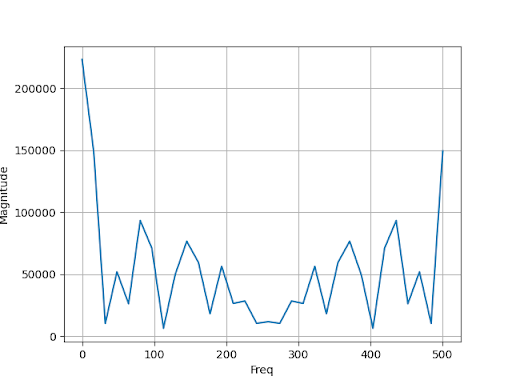
\includegraphics[scale = 0.75]{/imgs/fft_output.png}
    \caption{Output from the FFT Algorithm}
\end{figure}

\section{Visualization}
\par So far what I have done is create our serial fractal visualizer in C utilizing OpenGL's framework. Currently our images are being generated via a modified julia set algorithm to incorporate mobility with our “camera”. In other words you can zoom in/out and move the camera around. In addition there are also keybinds mainly for debugging, and finding values that work well for image generation. They do however also allow for exploration of the fractal that is being generated. So in a sense our visualization tool is multifunctional. I have also modified our animation function to utilize values from the fast fourier transform. These values are currently being used as a modifier for the values responsible for the generation of our fractal/visual. I tried having those values be the actual input to our fractal generation algorithm, and also tried scaling them. This However illustrated jarring results and will require further tuning. I plan on solving this by normalizing our values and messing with how the values are scaled to get cleaner results. So for now the extracted values from the FFT algorithm are being used as modifiers for our algorithm. A demonstration of the visuals can be seen at \url{https://www.youtube.com/watch?v=gugts8mUX-U}. In addition some more fractals generated from my algorithm can be seen below.  I have also spent some time thinking about how to visualize the colors in our algorithm and started messing with that. The colors correspond to the current iteration of our julia set which gives some really pretty, and some really trippy results. This is important because I hope to maintain that functionality once cuda is being utilized.

\par Most of the obstacles that were encountered pertained to OpenGl. I did have to learn a little bit about how it worked but that wasn’t too much of an issue as I have had some prior experience with graphics. Another issue as I hinted to above is how the values outputted from the FFT algorithm are interpreted. It was initially so bad I ended up giving myself a migraine. So I will only show our algorithm exactly correlating to the output of the FFT when I have got that working and it’s not painful to look at. I also had some issues running the visual side of the program on my desktop at home which is running windows as opposed to my laptop running linux. This will require some more research but for now i’ll write it up as I configured something wrong on my Desktop.
\par In terms of the original proposal I feel like this is almost exactly what I was thinking. Some modifications are going to have to be made to how values are interpreted from the FFT output but that shouldn’t be too much of an issue. 
\par In order to wrap up this portion of our project, it mostly comes down to implementing cuda, and tuning variables to get aesthetically pleasing and not jarring images. So In terms of finishing by the deliverable due date I think we’ll be ok on the visual side of things as I do feel a little ahead of schedule as of writing this.
\begin{figure}[!hbt]
    \centering
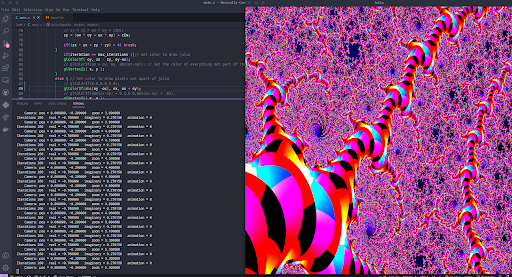
\includegraphics[scale = 0.75]{/imgs/v1.png}
\caption{Julia Set image where the non julia set parts correspond to values in an iteration. 
This could have some cool results in the final version.}
\end{figure}

\begin{figure}[!hbt]
    \centering
    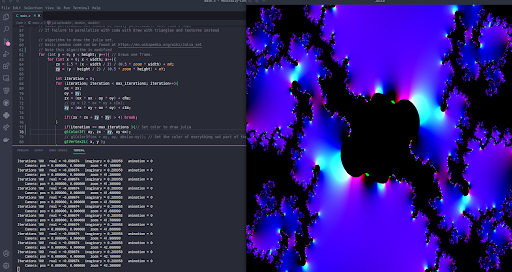
\includegraphics[scale = 0.75]{/imgs/v2.png}
    \caption{Another example of the julia set showcasing the functionality of the camera.
    The camera gives us more ways to generate an image. Might also be an interesting test case
    when it comes to using cuda.}
\end{figure}


\begin{figure}[!hbt]
    \centering
    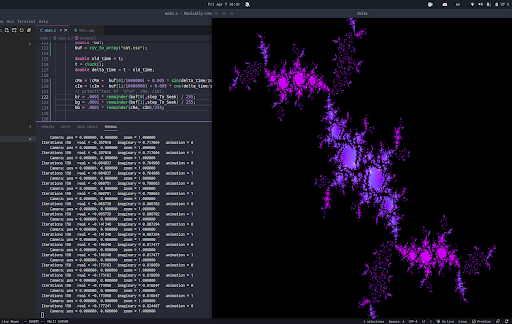
\includegraphics[scale = 0.75]{/imgs/v3.png}
    \caption{Another example of the image generation attempting to showcase the animation,
    and the creative images we can get from the output of our FFT algorithm.}
\end{figure}

\pagebreak
\begin{thebibliography}{9}
\bibitem{wikipedia} \url{https://en.wikipedia.org/wiki/Julia_set} 
\bibitem{Himanshu4746} \url{https://github.com/Himanshu4746/Morphy}
\bibitem{KyleSmith19091} \url{https://github.com/KyleSmith19091/Fourier-from-WAV-file/blob/master/Main.cpporphy}
\end{thebibliography}

\end{document}